\Chapter{Koncepció}

A fejezet egyik célja bemutatni a program létrehozásához alkalmazott technológiát: a Lua programozási nyelv alapvető tulajdonságait, sajátosságait.
Ezen kívül ismertetem a programtól elvárt működést részleteibe menően.
Megvizsgálom a jelenleg elkészítendő eszközhöz hasonló, Interneten fellelhető alternatívákat, továbbá OpenVPN esetében összehasonlítom a már elérhető OpenVPN Access Serverrel szemben a saját eszközöm koncepcióját.

A Lua egy már régóta használt programozási nyelv. Rövid történetét, működését, tulajdonságait \myaref{sect:used_language} alfejezetben mutatom be.
Dolgozatomhoz előnyös választásnak bizonyult, hiszen az így elkészült eszköz nem korlátozódik egyetlen platformra, lehetőséget biztosítva a későbbi, több platformot támogató továbbfejlődésre is.
Ezen kívül szkriptnyelvekre jellemző módon egyszerűségéből adódóan ideális a tervezett programhoz hasonló eszközök létrehozására. Úgy gondolom, hogy szintaxisa könnyen értelmezhető, továbbá felépítése is könnyen átlátható.

A dolgozatomban részletesen kifejtem a Lua sajátosságait, melyeket szükséges volt elmélyülten tanulmányoznom ahhoz, hogy elkészítsem az implementációmat.
Többek között kifejtem a metatáblák működésének elvét és használhatóságát, osztályok és öröklődések implementációját, konstruktort és objektum példányosítást, destruktort, és az osztályokon belüli láthatósági szabályokat.

A \myref{sect:how_it_should_work} alfejezetben kifejtem a programtól elvárt működést, ahogy a megvalósítás előtt megterveztem.
Ebben teljeskörűen felsorolom és részletezem, mik azok, amiket az eszközömnek tudnia kell.
Így például részletezem az OpenVPN szerver, a webszerverek, a Linux tűzfal kezelésének módját, és az ezeken belül elvárt funkcionalitásokat.
Külön foglalkozom a chroot és tls-crypt jelentésével és lényegével.

A fejezet végén ismertetem a tervezett programhoz hasonló funkcionalitást tartalmazó alternatívákat \myaref{sect:similar_apps} alfejezetben.

\Section{Felhasznált programnyelv}
\label{sect:used_language}
A program elkészítéséhez a felhasznált programnyelv a Lua, tesztelésre és az implementációra az 5.3.5 verziót használtam.

A \textbf{Lua} egy könnyű, magas szintű programozási nyelv, amelyet főképp az egyszerűen beágyazhatóság jegyében fejlesztettek ki. A legelső verzióját 1993-ban adták ki. Cross-platform, mivel implementációja ANSI C-ben íródott. Saját virtuális géppel és bytecode formátummal rendelkezik. A nyelv logója \myaref{fig:lua_logo} ábrán látható.

\pagebreak

\begin{figure}[h]
\centering

\includegraphics[scale=0.1]{images/Lua-Logo.svg}
\caption{A Lua logója \cite{lua_logo}}
\label{fig:lua_logo}
\end{figure}

A szkriptek futtatás előtt bytecode-ra fordítódnak át, majd úgy kerülnek átadásra az interpreternek. Mi magunk is lefordíthatjuk a Lua forráskódunkat a luac bináris segítségével.
Ezt akkor szokták megtenni, ha fel akarják gyorsítani a szkript futását, vagy ha nem szeretnék, hogy a forráskód is hozzáférhető legyen.

Támogat többféle programozási paradigmát is, azonban ezek nincsenek előre implementálva, viszont a nyelv lehetőséget ad arra, hogy implementáljuk őket. Például öröklődést, osztályokat metatáblák használatával tudunk megvalósítani. \cite{ooplua}

Széleskörű C API található felhasználásához, azonban nem csak erre a nyelvre korlátozódik az API használatának lehetősége, többféle függvénykönyvtár is készült a C API-hoz, a legtöbb azonban a C++ nyelvhez készült (például sol). \cite{sol_vs_other_bindings} 

Az interpreterje önmagában eléggé jó teljesítménnyel rendelkezik, jónéhány teljesítménymérés kimutatása szerint a Lua élvonalon jár teljesítmény szempontjából az interpretált szkriptnyelvek között. Nem csak végletekig-csiszolt "teljesítménymérésre szánt" programokban jó a teljesítménye, hanem a való életben való felhasználása közben is. Nagyobb sebességért a LuaJIT branchet is lehet használni.

A \textbf{LuaJIT} a Lua olyan verziója, amely Just-In-Time compilert tartalmaz, alapjaiban is gyorsabb, mint a Lua. A \myref{fig:luajit_logo} ábrán látható a lógója.

\begin{figure}[h]
\centering

\includegraphics[scale=0.15]{images/luajit-logo.jpg}
\caption{A LuaJIT logója \cite{luajit_logo}}
\label{fig:luajit_logo}
\end{figure}

A LuaJIT bytecode formátuma teljesen más, mint az eredeti Lua-é, gyorsabb az instrukciók dekódolása. A virtuális gépe is közvetlenül Assembly-ben íródott. A LuaJIT implementáció szinten nem kötődik hivatalosan a Lua programnyelvhez, attól független, más emberek fejlesztik. \cite {luajit}

A Lua programnyelvhez csomagkezelő is készült, amelyet LuaRocksnak hívnak, funkcionalitása hasonló a NodeJS \texttt{npm} csomagkezelőjéhez.

Előszeretettel használják a játékfejlesztők is, több neves játékban is előfordul, például World of Warcraft, PayDay 2, Saints Row széria, Crysis, Roblox, FiveM, MTA:SA. \cite{usageoflua}

\pagebreak

\Section{Metatáblák}
\label{sect:metatables}
Az előző szekcióban kifejtettem, hogy néhány programozási paradigma nincs előre implementálva, ezeket nekünk kell implementálunk. Öröklődést, osztályokat metatáblák segítségével tudunk implementálni.
A nyelvben minden táblának és userdatának lehet metatáblája. Az userdata típus adatok tárolására szolgál, a C API készíti, és az eltárolt adatok memóriacíme alapján működik (ez lehet akár az alap Lua IO függvénykönyvtár által megnyitott fájlok handleja, amelyek garbage collect esetén bezáródnak a \detokenize{__}\textbf{gc} metametódus segítségével; vagy például játékok esetében akár játékosadat, járműadat).

A metatábla egy olyan szokványos Lua tábla, amely meghatározza bizonyos műveletek viselkedését. Értelemszerűen egy metatáblát több táblára is fel lehet használni. A metatáblák legközelebbi rokonjai véleményem szerint a JavaScript nyelv Proxy-jai, azonban hasonlítanak a C++ nyelvben használt operátor túlterhelésre is. 

A metatáblákban találhatóak meg a metametódusok, amelyek meghívódhatnak bizonyos műveletekkor. Nevük két alsóvonallal kezdődnek, majd a metametódus neve követi. Például: \detokenize{__}\textbf{add}.

A metatáblák beállíthatóak a \textit{setmetatable} funkcióval, továbbá lekérhetőek a \textit{getmetatable} funkcióval. A metatáblákon belüli értéklekérésre célszerű a \textit{rawget} funkciót használni, ez kikerüli a további metatáblákat az értéklekéréskor.

Alapvetőleg csak tábláknak és userdata-knak van metatáblájuk. Minden más típusú adat saját \textit{-a típusának megfelelő-} metatáblát használ (például van külön számoknak, szövegeknek, satöbbi). Alapvetőleg egy értéknek nincs metatáblája, viszont például a beépített string függvénykönyvtár hozzáad a szöveg típusú értékeknek saját metatáblát, ezzel használható például a string:sub, string:gsub funkció is.

Néhány érdekesebb, akár a program által is felhasznált metametódusok:
\begin{itemize}
	\item \detokenize{__}\textbf{add}: hozzáadás művelete. Ha bármelyik operandus nem szám (és nem is szöveg, ami számot tartalmaz), akkor a Lua a metametódusokhoz nyúl, és ekkor próbálja ezt a metódust meghívni. Ha egyik operandusnál sem találja meg a metametódust, akkor hibát dob. A metametódus paraméterei a két operandus, és a funkciómeghívás végeredménye lesz az összeadás eredménye.
	\item további matematikai műveletek (\detokenize{__}\textbf{sub}, \detokenize{__}\textbf{mul}, \detokenize{__}\textbf{div}, \detokenize{__}\textbf{mod}, \detokenize{__}\textbf{pow}, \detokenize{__}\textbf{unm}, \detokenize{__}\textbf{idiv}): hasonlóan működnek az \detokenize{__}\textbf{add} metódushoz. Bitszinten is elérhetőek a bitmetódusok felülírása (például or, xor, and, not, satöbbi).
	\item \detokenize{__}\textbf{concat}: az összefűzés (Luaban: ..) művelete. Hasonló az \detokenize{__}\textbf{add} metametódushoz, ellenben ha bármelyik operandus nem szám és nem is szöveg (vagy szám alapú szöveg), máris megpróbálja az interpreter meghívni a metametódust.
	\item \detokenize{__}\textbf{len}: a hossz lekérdezés művelete (Luaban: \#). Ha az objektum nem szöveg, akkor ez a metódus kerül meghívásra. Ha nincs ilyen metódus, és az objektum egy tábla, akkor az alap hossz lekérdezés operátor lép működésbe. A meghívás return value-ja a visszaadott érték.
	\pagebreak
	\item \detokenize{__}\textbf{index}: Az egyik véleményem szerint legtöbbször felülírt metametódus. Alapját adja az OOP programozásnak a nyelvben. \texttt{\detokenize{obj[key]}} alapú értéklekérdezéskor hívódhat meg. Több esetben is meghívódhat:
		\begin{itemize}
			\item ha az objektumunk \textit{nem} tábla,
			\item ha az objektumunk tábla: akkor hívódik meg, ha a táblában nem található a keresett kulcsú érték.
		\end{itemize} Az index metametódus nem csak funkció lehet, hanem tábla is. Ha funkció, akkor meghívódik, két argumentummal: az \texttt{1.} argumentum maga az objektum lesz, a \texttt{2.} pedig a keresett kulcs. Tábla esetén pedig ott próbálja megkeresni az adott kulcsú értéket, ilyenkor ez a lekérdezés sem kerüli ki a metatáblák meghívódását.
	\item \detokenize{__}\textbf{newindex}: Működése hasonló az \detokenize{__}\textbf{index} metametódushoz. Akkor hívódik meg, amikor egy objektumon egy \texttt{\detokenize{obj[key] = value}} értéket beállítanak. A beállított metametódus szintén lehet funkció, vagy tábla, mint az \detokenize{__}\textbf{index} metametódusnál. Tábla argumentum esetén azon a táblán állítja be az értéket az interpreter, funkció esetén pedig meghívódik a következő argumentumokkal: objektum, key, value. Ekkor a meghívott funkció a \textit{rawset} funkció segítségével állíthat az objektumon értékeket (kikerülve a rekurzív metametódus meghívásokat).
	\item \detokenize{__}\textbf{call}: Meghívás operátor: \texttt{func(args)}. Akkor hívódik meg ez a metametódus, ha megpróbálunk meghívni egy nem funkció értéket. Ekkor func-ban kerül megkeresésre és meghívásra a metametódus (triviálisan csak akkor, ha létezik). Meghívása esetén func a legelső argumentum, a többi argumentum pedig az eredeti meghívás argumentuma (args). A meghívott funkció visszatérési értékei maga a meghívás visszatérési értékei is. Ez az egyetlen metametódus, amely több értékkel is visszatérhet.
	\item \detokenize{__}\textbf{gc}: Garbage collector metódus. Azelőtt hívódik meg, mielőtt a garbage collector felszabadítja az adott táblát/userdatat. Ez jó lehet például megnyitott fájlok, vagy bármi ilyen egyéb megnyitott erőforrások bezárására.
\end{itemize}

Jó szokás a lehető legtöbb metametódust definiálni az új metatáblánkban. A \detokenize{__}\textbf{gc} metametódus csak akkor működik, ha az összes metametódus sorban implementálva lett. Az összes metametódus részletesen megtekinthető a Lua Manualban.

Mivel a metatáblák átlagos táblák, ezért nem kötelező csak a metametódusokat tartalmazniuk, tartalmazhatnak tetszőleges adatokat is, amelyeket a bennük definiált funkciók felhasználhatnak. Például a \textit{tostring} funkció a metatáblában meghívja a \detokenize{__}\textbf{tostring} nevű funkciót (amely igazából egyedi metametódusnak is tekinthető), ha létezik, majd azt adja vissza, amit a funkció meghívásából visszakapott. \cite{metatable1}

\pagebreak

\Section{Osztályok, öröklődések implementálása metatáblák segítségével}

Az előző szekcióban megemlített \detokenize{__}\textbf{index} metametódussal tudunk osztályokat implementálni. Minden objektumnak van egy adott állapota, a tábláknak is.

A tábláknak van egy identitásuk, amely független a bennük tárolt értékektől, két tábla ugyan azokkal az értékekkel különböző objektumok is lehetnek, mindeközben egy tábla vagy userdata különböző értékekkel rendelkezhet különböző időkben, mégis ugyan az az objektum.

A tábláknak is van saját életciklusuk, amelyek függetlenek attól, hogy hol lettek létrehozva, vagy hogy ki hozta őket létre.

Az objektumoknak saját metódusai, műveletei vannak, csakúgy mint egy táblának.

\SubSection{Táblaműveletek, self kulcsszó}
A következő kódrészlet egy példa táblaműveletre:
\begin{lua}
Account = {balance = 0}
function Account.withdraw(value)
  Account.balance = Account.balance - value
end
\end{lua}
Ebben a példakódban létrehozunk egy Account táblát, amelyben van egy withdraw funkció. Ez a withdraw funkció a globális \texttt{Account} táblára vonatkozik, onnan fog értéket levonni. Ha megváltoztatjuk a nevét a táblának, vagy nil-lel tesszük egyenlővé, máris nem fog működni az alábbi kód.

A következő példakódban kiküszöböljük ezen problémákat, átnevezhetővé tesszük az objektumot, felülírhatóvá:

\begin{lua}
Account = {balance = 0}

function Account.withdraw(self, value)
  self.balance = self.balance - value
end 

a1 = Account; Account = nil

a1.withdraw(a1, 100.00)   -- OK

a2 = {balance=0, withdraw = a1.withdraw} -- itt figyelni kell arra, hogy az Account-ot mar nille raktuk (toroltuk), ezert a1-et hasznalunk 

a2.withdraw(a2, 260.00) -- OK

--alternativ hasznalati mod:
a1:withdraw(100.00) --OK
a2:withdraw(260.00) --OK
\end{lua}

A self paraméter bevezetésével már nem csak arra az objektumra/táblára érvényes a funkció, hanem bármelyik másra. Azonban ez a self paraméter úgymond saját magunk által implementált, kitalált.

Viszont ebben a nyelvben létezik a \texttt{self} kulcsszó, változó. A self változó mindig az adott objektumra/táblára mutat, vagyis önmagára. Ez egy nagy segítség az \textbf{OOP} implementálása során.

A Lua nyelvben a self változót kétféle képpen használhatjuk:

\hspace{10mm}\texttt{1}. megoldás: az előző példakódban tárgyalt 1. argument bevezetése. Abban a példakódban a self argumentumnevet igazából bármire kicserélhetjük, mivel a Lua nyelv akkor is oda fogja rakni első argumentként az objektumot, ha úgy használjuk, hogy: \texttt{Account:withdraw(value)}.

\hspace{10mm}\texttt{2}. megoldás:
\begin{lua}
Account = {balance = 0}

function Account:withdraw(value)
  self.balance = self.balance - value
end

a1 = Account; Account = nil

a1.withdraw(a1, 100.00)   -- OK

a2 = {balance=0, withdraw = a1.withdraw} -- itt figyelni kell arra, hogy az Account-ot mar nille raktuk (toroltuk), ezert a1-et hasznalunk 

a2.withdraw(a2, 260.00) -- OK

--alternativ hasznalati mod:
a1:withdraw(100.00) -- OK
a2:withdraw(260.00) -- OK
\end{lua}
Ebben az esetben a withdraw funkciót használva mindig a saját objektumunkra fog mutatni a self változó, kivéve akkor, ha két paraméter segítségével használjuk, és az első paraméter az objektum.

Most már az objektumjainknak van állapota, identitása, metódusai. Azonban nincsenek a klasszikus OOP nyelvekben megszokott osztályok, öröklődések, láthatósági szabályok.\pagebreak
\SubSection{Konstruktor, objektum példányosítás}
A korábban említett \detokenize{__}\textbf{index} metódus segítségével tudunk osztályainknak "konstruktort" írni:
\begin{lua}
Account = {}

function Account:new(o)
  o = o or {}   -- create object if user does not provide one
  setmetatable(o, self)
  self.__index = self
  return o
end

function Account:withdraw(value)
  if value > self.balance then error "insufficient funds" end
  self.balance = self.balance - value
end

function Account:deposit(value)
  self.balance = self.balance + value
end

a = Account:new{balance = 0}
a:deposit(100.00)
a:withdraw(100.00)

print(a.balance) --> 0
\end{lua}

Ebben az esetben létrehozunk egy Account táblát/objektumot, amelynek lesz \textit{new} funkciója, ez lesz a "konstruktorunk".

Ez a funkció úgy működik, hogy 1. argumentként kaphat egy állapot objectet/állapot táblát (ekkor a már meglévő objektum lesz állapotként felhasználva), vagy csinál egy teljesen üreset.

Az "o" táblára pedig saját magát, vagyis a jelenlegi objektumot (Account) állítja be metatáblának. Ezután pedig a self (Account) táblán beállítja az \detokenize{__}\textbf{index} metametódus értékét saját magára (tehát tábla lesz, nem funkció). Ennek segítségével minden definiált funkció működni fog úgy, hogy a self megmarad saját állapotként.

Így létrehozhatjuk az "a" változónév alatt eltárolt új objektumunk realizációját, amely most már bármire átnevezhető, bármikor törölhető. Az "a" objektumnak saját állapota lesz, saját belső változókkal, ugyanakkor az előre definiált \textit{deposit} és \textit{withdraw} funkciók ugyan úgy működni fognak. Ha az "a" objektumon meghívjuk ezeket a funkciókat, akkor a \textit{self} keyword magára az "a" táblára (objektumra) fog mutatni, így lesz saját állapota az objektumnak.

\SubSection{Destruktor}
A korábban említett \detokenize{__}\textbf{gc} metódus segítségével tudunk destruktort írni objektjeinknek, ez lefut, mielőtt a garbage collector felszabadítaná őket. Hasznos lehet olyan erőforrások bezárására, amelyek maguktól nem szabadulnak fel.
\pagebreak
\SubSection{Öröklődés}
Az előző, legutolsó példakódot felhasználva könnyedén tudunk öröklődést implementálni. Ne felejtsük el, hogy a \texttt{self} változó mindig önmagunkra mutat. Az alábbi példakódban megtekinthető az öröklődés mechanizmusa:

\begin{lua}
SpecialAccount = Account:new() --letrehozunk egy uj Account objektum peldanyt, amelyet SpecialAccountkent nevezunk el. Azonban a SpecialAccount minden olyan tulajdonsaggal rendelkezik, mint az Account.

s = SpecialAccount:new{limit=1000.00, balance=0} --Ezert lehet ugyan ugy peldanyositani ot is, mint az Account objektumot.
s:deposit(100.00) --ebben az esetben a self parameter az "s"-re mutat. Az "s" metatablaja pedig SpecialAccount lesz. Ezaltal az "s" orokli a SpecialAccountot, ami pedig orokli az Accountot.
--mivel a Lua nem talalja meg a deposit funkciot SpecialAccountban, ezert tovabb megy, es az Accountban megtalalja, meghivja azt. Azonban a metodusok felulirhatoak az uj objektumban:

function SpecialAccount:withdraw(value)
  if value - self.balance >= self:getLimit() then
    error "insufficient funds"
  end
  self.balance = self.balance - value
end

function SpecialAccount:getLimit()
  return self.limit or 0
end

s:withdraw(200.00) --[[mostmar a Lua interpreternek nem kell az Accountig visszamennie, mivel a SpecialAccountban a withdraw definialva van, ezert azt fogja meghivni. 
a Lua nyelv erdekessege, hogy nem kell uj osztalyt letrehozni annak, hogy kulonleges viselkedest definialjunk egy adott objektumra. Felul lehet irni az "s" objektum funkcioit is, hogy maskepp viselkedjenek]]
function s:getLimit()
  return self.balance * 0.10
end

s:withdraw(200.00) --ekkor a Lua a SpecialAccount withdrawjat fogja meghivni, viszont a getLimit funkcio a "self" miatt az "s" objektum felulirt funkcioja lesz, azt fogja meghivni.
\end{lua}
\pagebreak
\SubSection{Láthatósági szabályok osztályokon belül}
A többi nyelvhez hasonlóan itt is lehet alapszintű láthatóságot beállítani az osztályokon belül. Alapvetőleg ez sincs implementálva a nyelvben, azonban a Lua flexibilis nyelvnek készült, ezáltal mi magunk elkészíthetjük. Egy tábla helyett két táblát fogunk használni egy objektum reprezentálására:
egyet az állapotára, a másikat pedig interfészként, amelyen keresztül interaktálni tudunk vele. A belső \textit{-állapot-} táblát pedig csak a definiált funkciók érik el. Az előzőekhez hasonló példakód:

\begin{lua}
function newAccount(initialBalance)
  local self = {balance = initialBalance, LIM = 10000.00}

  local withdraw = function(value)
    self.balance = self.balance - value
  end

  local deposit = function(value)
    self.balance = self.balance + value
  end
	
  local extra = function()
    if self.balance > self.LIM then
      return self.balance * 0.10
    else
      return 0
    end
  end

  local getBalance = function() return self.balance + extra() end

  return {
    withdraw = withdraw,
    deposit = deposit,
    getBalance = getBalance
  }
end

acc1 = newAccount(100.00)
acc1.withdraw(40.00)
print(acc1.getBalance())     --> 60
\end{lua}
Ebben a példakódban a \textit{newAccount} a konstruktorunk, amely vár egy értéket, hogy a bankszámlánk mennyi pénzzel indul. Létrehoz egy belső táblát, amely csak a belső scopen belül létezik, self néven. Ez lesz az állapot tábla. Minden benne tárolt érték "private" láthatóságúak. 

A többi funkciót ugyan abban a belső scopeban definiálja, ezért alapvetőleg nem is lennének elérhetőek kívülről, azonban egy új tábla hozódik létre, az interfész tábla return valueként, mely elérhetővé teszi ebben a belső scopeban létrehozott funkciókat.

Ebben az esetben a \texttt{self} kulcsszó nem a szokványos változó lesz, hanem egy elnevezett változó a belső scopeban. 

\pagebreak

A definiált funkciók folyton arra a "self" változóra fognak hivatkozni, amelyet mi definiáltunk, ezért nem fogad extra argumentet arról, hogy melyik objektum tartalmazza az állapotot.

Emiatt a ":" használatát mellőznünk kell, csak a "." használatával tudjuk használni a funkciókat. Definiáltunk egy olyan funkciót is, amely szintén "private" láthatóságú, ez az \textit{extra} nevű funkció. \cite {classes}

\Section{Programtól elvárt működés}
\label{sect:how_it_should_work}

A program a szerverek konfigurációja közben igyekszik a jelenleg elérhető legjobb biztonsági megoldások alkalmazására, titkosítás, SSL beállítás és egyéb dolgok terén (például chroot, tls-crypt).

Az OpenVPN Community szervert a program tudja kezelni, telepíteni. A telepítést az apt-get beépített segédprogrammal végzi. Kezelni tudja az alábbi dolgokat:
\begin{itemize}
	\item kliensek létrehozása (kulcs alapú), törlése (kulcs esetén revoke),
	\item kliensek számára személyre szabott .ovpn config generálás,
	\item init.d beállítások, az eredeti daemon beállítása automatikus indításra,
	\item külön user létrehozása a szerver futtatására,
	\item tls-crypt használata az üzenetek titkosításához (a tls-crypt leírása itt olvasható: \ref{ref:tls-crypt}),
	\item chroot használata a szerver futtatásához a megnövelt biztonság érdekében (a chroot leírása itt olvasható: \ref{ref:chroot}).
\end{itemize}
Fontos kiemelni, hogy az OpenVPN implementáció a server.conf config fájlt módosítja, azonban nem ellenőrzi kifejezetten a config fájl helyességét, így nem tud config fájlt javítani sem.

Apache2 és nginx webszervert is tud kezelni a program, ebbe beletartozik:
\begin{itemize}
	\item telepítés apt-gettel,
	\item honlap hozzáadása külön directoryval,
	\item honlap törlése,
	\item SSL certificate kezelés Let's Encrypton belül certbot segítségével, a certbot snapd-n keresztül települ; up-to-date SSL beállításokra törekszik a program,
	\item külön user a daemonoknak mind Apache2, mind nginx esetében,
	\item a jelenlegi implementáció csak statikus weboldalakat támogat, ezért egy user van egy egész daemonnak, nincs külön weboldalanként user\\PHP/bármilyen szerveroldali kiegészítő esetén célszerű különböző usereket használni weboldalanként.
\end{itemize}

Szintén konfigurációbeállítást végez a program a webszerverek esetében is, teljes mértékben nem tudja a konfigurációs fájlok helyességét ellenőrizni, sem megjavítani őket, ha hibásak.

Tűzfal gyanánt az iptables nevű beépített Linux segédprogramot tudja kezelni.

\pagebreak

Iptables funkcionalitások:
\begin{itemize}
	\item telepítés apt-gettel ha nincs fent,
	\item IPv4 támogatás,
	\item port nyitás, zárás,
	\item bizonyos portra csak bizonyos IP-ről csatlakozás engedélyezése,
	\item bizonyos IP cím felé csak bizonyos kimeneti portok felé kimenő kapcsolat engedélyezése,
	\item nyitott portok listázása,
	\item zárt portok listázása,
	\item engedélyezett kimenő kapcsolatok listázása,
	\item OpenVPN szerverhez köthető NAT Forward listázása, kezelése.
	\item A fenti szabályok korlátozhatóak az egyes network interfacekra.
	\item Szabályellenőrzés, például ha engedélyezünk egy portot, és nincsenek letiltva a nem engedélyezett bejövő kapcsolatok, akkor figyelmeztetés.
	\item Ki-be kapcsolható togglek:
		\begin{itemize}
			\item Bejövő forgalom csak az engedélyezettek közül jöhet be - ekkor ellenőrzi, hogy SSH port az engedélyezettek között van-e, és ha nincs, akkor figyelmeztet.
			\item Kimenő forgalom csak az engedélyezettek felé mehet ki.
		\end{itemize}
\end{itemize}

\SubSection{Mi az a tls-crypt?} \label{ref:tls-crypt}
A tls-crypt egy OpenVPN beállítás, amely lehetővé teszi, hogy az összes csomag digitálisan legyen aláírva, továbbá titkosítva akár szimmetrikus eljárásokkal. Ez a key-exchange előtt is már alkalmazásra kerül. \cite{openvpnmanual}
Többféle előnye is van:
\begin{itemize}
	\item nehezebb megkülönböztetni az OpenVPN csomagjait,
	\item több biztonságot ad azzal, hogy a TLS kapcsolódást is titkosítja már,
	\item közbeékelődéses támadás ellen is védhet, továbbá túlterheléses támadások ellen is.
\end{itemize}

\SubSection{Mi az a chroot?} \label{ref:chroot}
A chroot\texttt{(const char *path)} egy olyan C API hívás, amely a jelenlegi gyökérkönyvtárat átváltoztatja arra, amelyet az első argumentben megadnak neki. Ez azt jelenti, hogy a jövőben az összes fájlművelet ehhez a gyökérkönyvtárhoz lesz relatív, abban az esetben, ha \texttt{/}-lel kezdődik a megnyitott fájl pathja. Kiterjed a mostani és az az összes child-processzre is a változtatás. \cite{chroot}

Csak privilegizált programok tudják általában ezt a C API hívást meghívni. Vigyázni kell programozói szempontból a használatával, mivel ez igazából csak a védelem egy alapját adhatja meg, bizonyos módszerekkel kikerülhető.

\Section{Hasonló alkalmazások}
\label{sect:similar_apps}
Az Internet sokaságában sok hasonló funkcionalitást implementáló alkalmazást lelhetünk fel.

\SubSection{Apache2 és nginx}
Többféle neves implementáció is létezik az Apache2 és nginx kezelésére. A webszerverek logói \myaref{fig:webservers_logo} ábrán láthatóak.

\begin{figure}[h]
	\centering
	\begin{subfigure}{.5\textwidth}
		\centering
		
\includegraphics[scale=0.35]{images/apache_httpd_logo.png}
		\caption{Az apache logója \cite{apache_logo}}
	\end{subfigure}%
	\begin{subfigure}{.5\textwidth}
		\centering
		
\includegraphics[scale=0.35]{images/nginx_logo.png}
		\caption{Az nginx logója \cite{nginx_logo}}
	\end{subfigure}%
	\caption{A webszerverek logói}
	\label{fig:webservers_logo}
\end{figure}

Legelőször személy szerint a \textbf{VHCS} vagyis a Virtual Hosting Control Systemmel találkoztam jópár évvel ezelőtt. A VHCS már nincs aktívan fejlesztve, az utolsó kiadott verzió belőle a 2.4.8-as verzió, amely 2009-ben jelent meg. \cite{vhcs} Többféle szervert is tudott kezelni, néhány ezek közül: Apache, ProFTPD, MySQL, Bind. A későbbiekben az ispCP projekt erre épült. \cite{ispcp} 

Az \textbf{ispCP} projektből alakult ki az \textbf{i-MSCP}, amelynek a legutolsó kiadott verziója 2018-ban lett kiadva \cite{imscp}. Ez már több featureval rendelkezik:
\begin{itemize}
	\item kezeli az Apache2-t és az nginx-et egyaránt,
	\item támogatja a PHP szerver oldali webfejlesztést,
	\item kezeli a bind DNS szervert,
	\item kezel Mail Transfer Agentet,
	\item kezel Mail Delivery Agentet,
	\item kezel adatbázisszervereket,
	\item kezel FTP-szervereket,
	\item pluginnal való bővítés lehetősége adott.
\end{itemize}
Azonban jelenleg a dolgozat írásakor a projektet nem fejlesztik aktívan. Az előzőleg említett VHCS, ispCP és i-MSCP szerverkezelő implementációk mindannyian nyílt forráskódúak, ingyenesen felhasználhatóak, többnyire Linux alapú rendszerekre készültek.

A következő lehetséges implementáció az \textbf{ISPConfig}. Ez is szintén nyílt forráskódú, ingyenesen felhasználható, és Linux alapú rendszerekre készült. PHP-ban íródott. Legutolsó stabil verziószám: 3.2.11, amely 2023. augusztus 8.-án lett kiadva. \cite{ispconfig}

Széleskörű funkcionalitással rendelkezik, sok daemont, szervert kezel \cite{ispconfig2}:
\begin{itemize}
	\item webszerverek közül az Apache2-t és az nginx-et egyaránt,
	\item támogatja a PHP-t is, azonban külön fel kell rakni és beállítani a felületen,
	\item SMTP szerverek közül a postfix-et,
	\item POP3/IMAP szerverek közül a Dovecot-ot,
	\item FTP szerverek közül a PureFTPD szervert,
	\item DNS szerverek közül a bind, PowerDNS szervert,
	\item többféle adatbázisszervert támogat: MariaDB és MySQL,
	\item többféle felhasználói nyelvet is támogat.
\end{itemize}

A következő táblázatban a myVestaCP implementáció kerül összehasonlítása az ISPConfig-gal.
A \textbf{myVestaCP} szintén nyílt forráskódú, a \textbf{vestaCP} forkolt, továbbfejlesztett változata. A két implementáció összehasonlítása \myaref{tab:ispconfig_vs_myvestacp} táblázatban látható.

\begin{table}[h]
\centering
\caption{ISPConfig \cite{ispconfig2} összehasonlítása myVestaCP-vel \cite{myvestacp}}
\label{tab:ispconfig_vs_myvestacp}
\begin{tabularx}{\linewidth}{l|L|L}
 & ISPConfig & myVestaCP \\
\hline
Ingyenes & igen (kivéve Dokumentáció \cite{ispconfig_doc}) & igen \\
\hline
Szerver kezelés támogatott OS & Kizárólag Linux support & Kizárólag Debian support \\
\hline
Kezelt szervertípusok & Web, SMTP, POP3/IMAP, webmail, FTP, DNS, SQL, tűzfal (iptables) & Web, SQL, DNS, POP3/IMAP, webmail, Antivirus, FTP, node.js web, tűzfal (iptables, fail2ban) \cite{vestacpdocs} \\
\hline
Támogatott nyelvek & Többnyelvű & Angol, többi nem ismert \\
\hline
Web interface alapú & Igen & Igen \\
\hline
Testreszabhatóság & Léteznek hozzá modulok, pluginok & Léteznek hozzá modulok, pluginok, azonban nem annyira nagy a választék \\
\end{tabularx}
\end{table}

\SubSection{Tűzfal}
Tűzfalak terén a Linux rendszerekben a legelterjedtebb netfilter implementációk jelenleg az iptables és az nftables. A netfilter logója \myaref{fig:netfilter_logo} ábrán látható.

\begin{figure}[h]
\centering

\includegraphics[scale=0.5]{images/netfilter-logo3.png}
\caption{A netfilter logója \cite{netfilter_logo} - ezt használja az iptables is.}
\label{fig:netfilter_logo}
\end{figure}

Az \textbf{iptables} legelső kiadása 1998-ban, a legutolsó stabil kiadása 2022. május 13.-án jelent meg. C-ben íródott. \cite{iptables}

Többféle táblát használ a parancsok feldolgozására, tud csomagokat szűrni (ki és bemenő, továbbá átirányított csomagokat), csomagok tartalmát módosítani, átirányítani. Tud NAT-ot is implementálni. \cite{iptables_man}

Az \textbf{nftables} a Linux kernel 3.13-as verziójától érhető el, pontosabban 2014 január 19.-e óta. Az nftables néhány iptables-hez köthető maradandó örökséget cserél le, tudja többnyire ugyan azt a funkcionalitást, mint az iptables. Előnye az iptables-hez képest, hogy kevesebb kód duplikációval rendelkezik, és könnyebb az új protokollokra való kibővítése. \cite{nftables}
Jobban skálázható is, jobb a teljesítménye az iptablesnél, főleg akkor, ha például iptables-ban sok saját magunk által definiált chain-t (láncot) használtunk.

Jónéhány Linux disztribúcióban, például a Debian újabb verzióiban egyszerre mindkettőt használhatjuk. Az \texttt{iptables -V} parancsot lefuttatva megnézhetjük, hogy milyen iptablessel dolgozunk. Az újabb verziókon az iptables igazából nftables backendet használ, ezt a következőképp láthatjuk \myaref{fig:iptables_nftables} ábrán.
\begin{figure}[h]
\centering
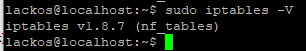
\includegraphics[scale=1.0]{images/iptables_nftables.png}
\caption{Debian 11-es rendszeren használt iptables, amely nftables backenddel dolgozik}
\label{fig:iptables_nftables}
\end{figure}

Létezik iptables szabálylánc konvertáló program is, amellyel meglévő szabályainkat nftables szintaxisra konvertálhatjuk. 

Az elkészítendő program az \textit{iptables} backendet használja, mivel az a régebbi rendszereken is használható, továbbá még mindig elterjedt az \textit{nftables} mellett is. Többféle elterjedt tűzfal implementáció is van, amelyek az iptables-t használják fel, a következő \myref{tab:ufw_vs_firewalld} táblázatban kettőt fogok összehasonlítani

	\begin{table}[h]
	\centering
	\caption{ufw összehasonlítása firewalld-vel}
	\label{tab:ufw_vs_firewalld}
	\begin{tabularx}{\linewidth}{l|X|X}
	 & ufw & firewalld \\
	\hline
	Használatának módja & CLI, de létezik hozzá GUI is & CLI, de létezik hozzá GUI is \\
	\hline
	Ingyenes & igen & igen \\
	\hline
	Parancsok formátuma & egyszerű parancsokkal rendelkezik, angol parancsok könnyű paraméterezéssel \cite{ufw} & kevésbé felhasználóbarát, komplexebb parancsok \cite{firewalld_man}\\
	\hline
	Támogatott protokollok & TCP, UDP. A ping engedélyezéséhez már iptables szabályokat kell írni & /etc/protocols-ból támogatja az összeset, portnál TCP/UDP/sctp/dccp protokollt támogat \\
	\hline
	Testreszabhatóság & nincsenek hozzá pluginok & nincsenek hozzá pluginok \\
	\end{tabularx}
	\end{table}
	
\pagebreak

\SubSection{OpenVPN}
A következő \ref{tab:openvpn_apps} táblázatban a saját implementációmat, amely OpenVPN Community szervert használ, hasonlítom össze az OpenVPN Access Server-rel. Az OpenVPN logója \myaref{fig:openvpn_logo} ábrán látható.

\begin{figure}[h]
\centering

\includegraphics[scale=0.5]{images/openvpn-logo.png}
\caption{Az OpenVPN logója \cite{openvpn_logo}}
\label{fig:openvpn_logo}
\end{figure}

Fontos megemlíteni, hogy OpenVPN szerver menedzser implementáció több is létezik, létezik C\#-ban írt, létezik Bash Scriptben írt is. A minél nagyobb cross-platform támogatás lehetősége miatt azonban úgy gondolom mégis helyt áll a program létezése, a Lua nyelv egyszerűsége, nagyszerű cross-platform támogatása miatt. Értelemszerűen a Bash Script implementációk csak Linuxra korlátozódnak. GitHubon létezik web alapú interface is az OpenVPN Community Serverhez.

\begin{table}[h]
\caption{Az OpenVPN Access Server összehasonlítása saját implementációval}
\label{tab:openvpn_apps}
\begin{tabularx}{\textwidth}{l|L|L}
 & OpenVPN Access Server \cite{openvpnaccessserver} & Saját implementáció (OpenVPN Community) \\
\hline
Ingyenes & nem & igen \\
\hline
Kliens támogatott OS & Cross-platform & Cross-platform \\
\hline
Szerver kezelés támogatott OS & a legtöbb támogatott & kizárólag Linux support\\
\hline
User authentikáció módja & webes alapú felhasználónév-jelszó, PAM, LDAP \newline RADIUS, SAML, stb. Saját auth script is készíthető. & kizárólag kulcs alapú (ez bővíthető saját auth scriptekkel, továbbá pluginokkal, például PAM pluginnal). \\
\hline
Többfaktoros hitelesítés & beépített lehetőségek, továbbá pluginokkal bővíthető lehetőségek & saját auth scripttel kivitelezhető a 2FA, vagy akár pluginként \\
\hline
Access Control (ACL) & beépített lehetőségek & saját auth scripttel, vagy tűzfallal kivitelezhető \\
\hline
Tunnel átirányítás & beépített lehetőségek: full-tunnel és split-tunnel & megoldható a kliens konfigurálásával (a \texttt{route} program használatával), továbbá szerveroldali konfigurálással (redirect-gateway) \\
\end{tabularx}
\end{table}

\pagebreak

\begin{table}[h]
\caption{A \ref{tab:openvpn_apps} táblázat folytatása}
\label{tab:openvpn_apps2}
\begin{tabularx}{\textwidth}{l|L|L}
 & OpenVPN Access Server \cite{openvpnaccessserver} & Saját implementáció (OpenVPN Community) \\
\hline
Support & professzionális support ticketing rendszerrel & OpenVPN community fórum, Community Ticket report \\
\hline
Certificatek kezelése & automata, beépített tanusítványkezelés van, külső infrastruktúrát is lehet használni & saját, automatizált tanusítványkezelés \\
\hline
Kezelőfelület & webes alapú, command line & alapvetőleg command line, azonban webes alapú felület is lehetséges 3rd party szoftverekkel
\end{tabularx}
\end{table}
